\chapter{Fundamentação teórica}
\label{cap:fundamentacao-teorica}

Neste capítulo, serão apresentados os principais conceitos fundamentais para o
desenvolvimento deste trabalho. A Seção~\ref{sec:roguelike-roguelites} trata dos
aspectos históricos e mecânicas fundamentais dos gêneros \textit{roguelike} e
\textit{roguelite}.  Na Seção~\ref{sec:pcg_em_jogos}, discute-se a \gls{PCG},
abordando sua definição, objetivos, aplicações, vantagens, desafios e técnicas
comuns. Por fim, a Seção~\ref{sec:llms} oferece uma descrição sobre os
\gls{LLM}s, considerando sua definição, evolução, arquitetura, treinamento,
capacidades e aplicação na \gls{PCG}.

\section{Roguelikes e Roguelites}
\label{sec:roguelike-roguelites}

O gênero \textit{roguelike} compreende uma categoria de jogos de \gls{RPG}
eletrônicos caracterizados por uma série de mecânicas distintas, das quais a
morte permanente e a geração procedural de níveis são as mais proeminentes. O
termo deriva diretamente do jogo seminal \textit{Rogue}\footnote{Artigo sobre
	\textit{Rogue} no site \textit{RogueBasin}, uma das principais \textit{Wikis} de
	\textit{Roguelikes} tradicionais (Acesso em: 23 jan. 2026): \url{https://www.roguebasin.com/index.php/Rogue}}\footnote{Manual
	do jogo Rogue (Acesso em: 23 jan. 2026): \url{https://britzl.github.io/roguearchive/files/misc/EpyxRogueDOSManual/manual.htm}},
desenvolvido por Michael Toy, Glenn Wichman e Ken Arnold e lançado em 1980.
\textit{Rogue} surgiu em um contexto no qual jogos de aventura baseados em
texto, como \textit{Colossal Cave Adventure}, e \gls{RPG}s de mesa, como
\textit{Dungeons \& Dragons}, eram populares, mas a representação gráfica e a
interatividade dinâmica em computadores pessoais ainda estavam em seus estágios
iniciais \cite{harris2020exploring}.

Em \textit{Rogue}, o jogador assume o papel de um aventureiro explorando uma
masmorra perigosa com o objetivo de recuperar o Amuleto de \textit{Yendor} e retornar à
superfície. O jogo utilizava caracteres no formato \gls{ASCII} para representar
graficamente o personagem do jogador (geralmente um '@'), monstros
(representados por letras diversas), itens e o layout da masmorra, como
ilustrado na Figura~\ref{fig:rogue}. Esta abordagem visual, embora primitiva
para os padrões atuais, era inovadora por permitir uma representação espacial do
ambiente do jogo, que era gerado aleatoriamente a cada nova partida, uma
característica fundamental que definiria o gênero.

\begin{figure}[!ht]
	\centering
	\Caption{\label{fig:rogue} Screenshot do jogo \textit{Rogue}}
	\UFCfig{}{
		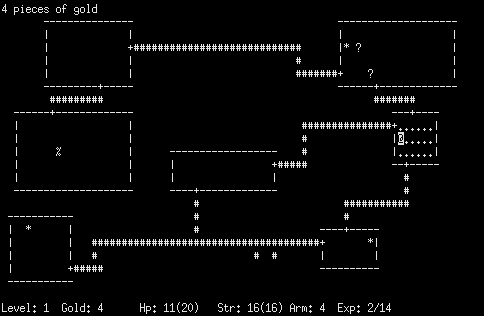
\includegraphics[width=0.8\textwidth]{figuras/screenshot_rougue.png}
	}{
		\Fonte{Disponível em: \url{https://en.wikipedia.org/wiki/Rogue_(video_game)}. Acesso em: 23 jan. 2026.}
	}
\end{figure}

O impacto de \textit{Rogue} foi significativo, estabelecendo as fundações para
um gênero que persistiria e evoluiria por décadas \cite{harris2020exploring}.
Desenvolvido para terminais \textit{Unix} e utilizando a biblioteca
\textit{Curses}\footnote{\textit{Curses} (Acesso em: 23 jan. 2026): \url{https://www.ibm.com/docs/en/aix/7.2.0?topic=concepts-curses-library}}
para manipulação de tela, \textit{Rogue} introduziu avanços importantes não
apenas para os \gls{RPG}s de computador, mas para o gênero de jogos de PC em
geral. A geração procedural, a trama básica de exploração e retorno, e a
exibição baseada em texto tornaram-se características centrais e recorrentes nos
jogos que se seguiram e que se autodenominariam \textit{roguelikes}
\cite{harris2020exploring}.

Um dos pilares fundamentais do gênero \textit{roguelike} é a mecânica de
morte permanente. Essa característica implica que, quando o personagem do
jogador morre, todo o progresso naquela partida específica é perdido, e o
jogador deve recomeçar do zero. A morte permanente intensifica a tensão e o
valor de cada decisão tomada pelo jogador, pois um erro pode ter consequências
fatais e irreversíveis para aquela sessão de jogo. Este ciclo de tentativa,
falha e aprendizado é central para a experiência \textit{roguelike}, forçando os
jogadores a internalizar as mecânicas do jogo e a desenvolverem suas próprias
habilidades e estratégias, em vez de dependerem apenas da progressão virtual do
personagem.

A natureza punitiva da morte permanente é frequentemente vista como um elemento
que torna as escolhas e os riscos mais significativos. Em muitos jogos de \gls{RPG}
tradicionais, a morte do personagem é uma inconveniência temporária, resolvida
com o carregamento de um jogo salvo. Nos \textit{roguelikes} clássicos, no
entanto, a perda do personagem significa o fim daquela jornada específica, e o
jogador leva consigo apenas o conhecimento adquirido para a próxima tentativa.
Este foco na habilidade do jogador, em detrimento da acumulação de recursos ou
níveis do personagem que persistem entre as mortes, é um diferencial marcante do
gênero \cite{bottaoh}.

De forma complementar à morte permanente, a \gls{PCG} é o outro pilar essencial
dos \textit{roguelikes}. Em \textit{Rogue}, e em seus sucessores, os níveis da
masmorra, a localização de inimigos, itens e tesouros são gerados
algoritmicamente a cada nova partida.  Isso garante uma alta rejogabilidade,
pois cada sessão de jogo apresenta um desafio único e imprevisível. Mesmo os
desenvolvedores de \textit{Rogue} não poderiam prever a configuração exata de
uma masmorra, o que contribuía para a sensação de exploração genuína
\cite{short2017procedural}.

Por muitas décadas, o gênero \textit{roguelike} permaneceu um nicho, apreciado
por uma comunidade dedicada de fãs, mas foi nesta última década que ele emergiu
para o \textit{mainstream}, influenciando uma vasta gama de jogos independentes e até
mesmo títulos de grande orçamento \cite{Bycer2019RoguelikeDebate}. Com essa
popularização, surgiu o termo \textit{roguelite}\footnote{Debate sobre
	o significado do termo \textit{Roguelite} (Acesso em: 23 jan. 2026):
	\url{https://www.gamedeveloper.com/design/the-roguelike-debate----roguelikes-vs-roguelites}}
para descrever jogos que incorporam elementos chave dos \textit{roguelikes},
como a morte permanente e a geração procedural, mas que se desviam da fórmula
clássica, muitas vezes introduzindo sistemas de meta-progressão.  Essa
meta-progressão permite que certos desbloqueios, habilidades ou recursos sejam
carregados entre as partidas, suavizando a curva de dificuldade e oferecendo uma
sensação de progresso contínuo mesmo após a falha \cite{Albert2023Roguelites}.

\begin{figure}[!ht]
	\centering
	\Caption{\label{fig:deadcells} Dead Cells (2018)}
	\UFCfig{}{
		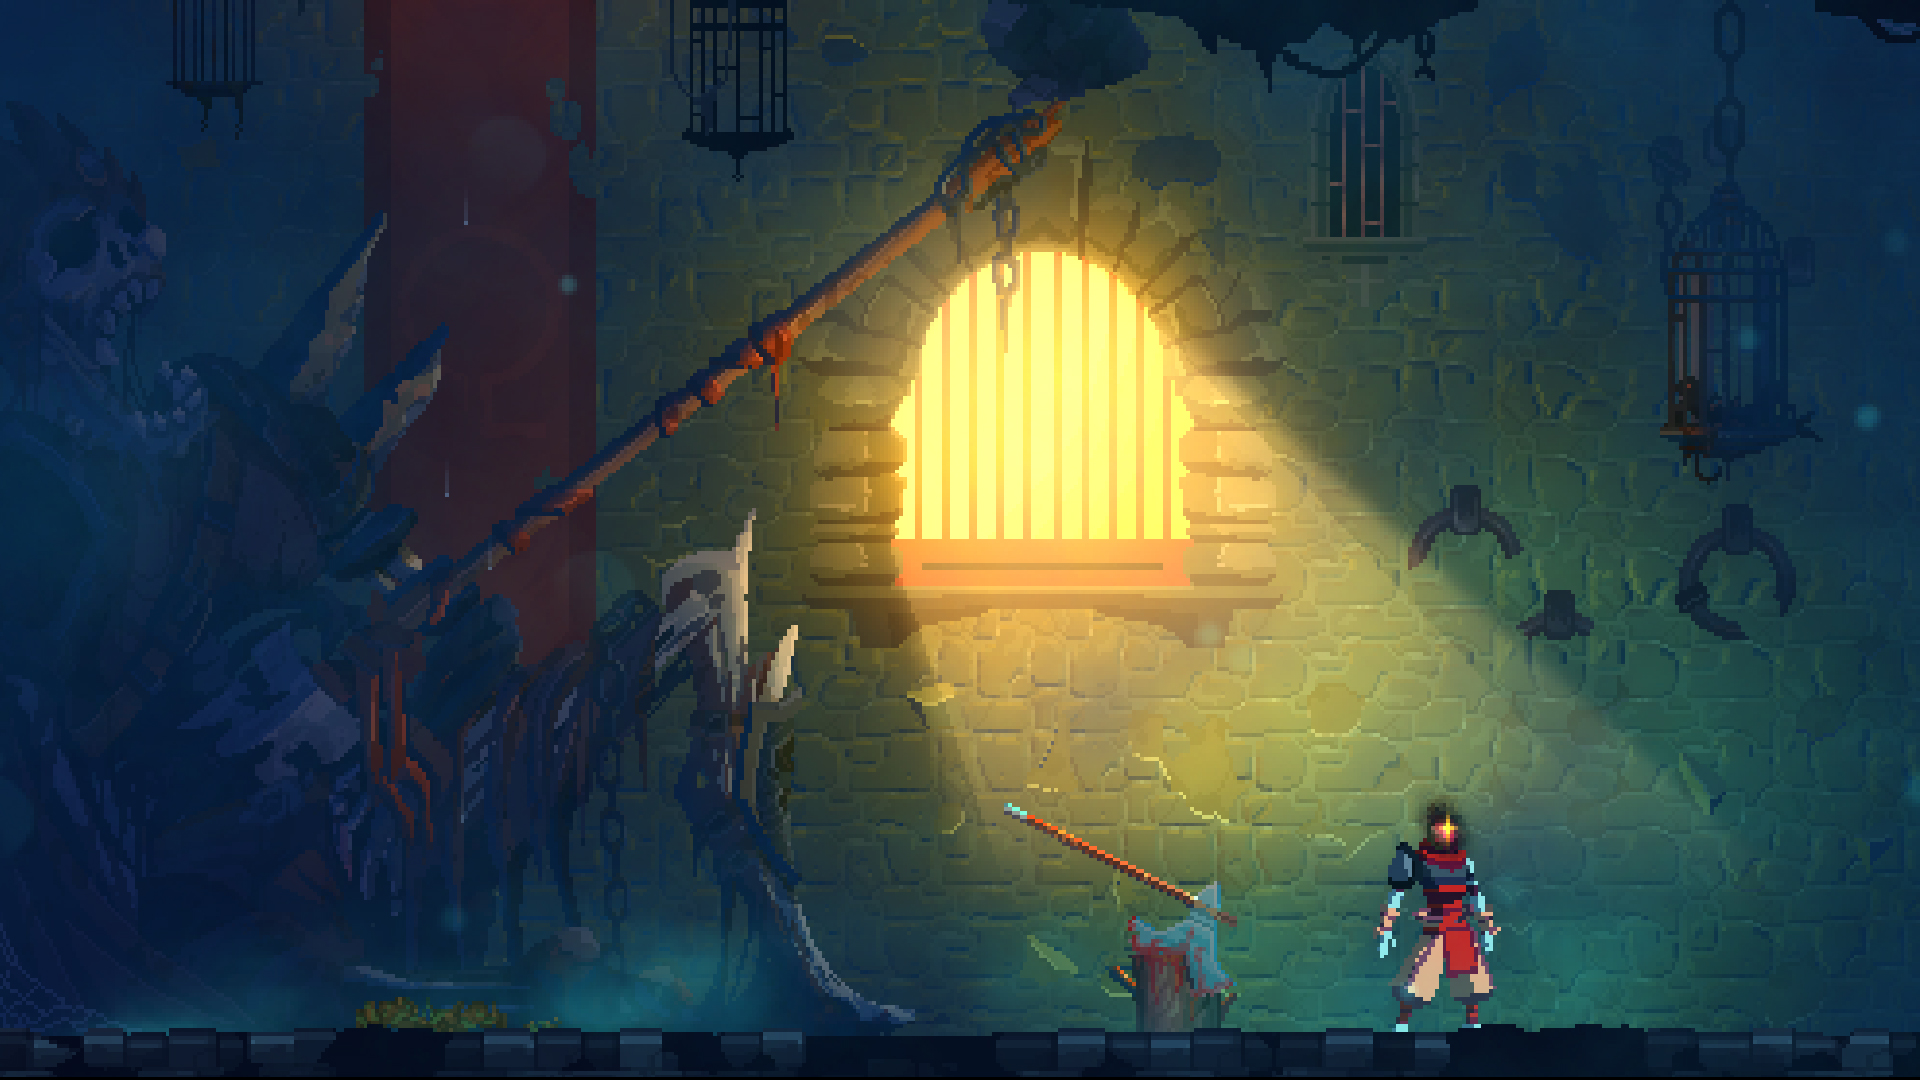
\includegraphics[width=0.8\textwidth]{figuras/dead_cell_2017.jpg}
	}{
		\Fonte{Disponível em: \url{https://store.steampowered.com/app/588650/Dead_Cells/}. Acesso em: 23 jan. 2026.}
	}
\end{figure}

Os \textit{roguelites} focam frequentemente em alcançar um final definido, em
contraste com os \textit{roguelikes} clássicos, nos quias o foco está mais na jornada
e na superação de desafios imediatos de cada partida. A persistência de
elementos entre as tentativas, como melhorias de atributos base, desbloqueio de
novas armas ou habilidades, mecânicas centrais em títulos como o visualmente
impactante \textit{Dead Cells} (Figura~\ref{fig:deadcells}), torna os
\textit{roguelites} mais acessíveis a um público mais amplo, que pode se sentir
frustrado pela natureza implacável da morte permanente total. Outros títulos
como \textit{Spelunky}\footnote{Site oficial do \textit{Spelunky} (Acesso em: 23 jan. 2026): \url{https://www.spelunkyworld.com/}}, \textit{FTL:
	Faster Than Light}\footnote{Site oficial do \textit{FTL:
		Faster Than Light} (Acesso em: 23 jan. 2026): \url{https://subsetgames.com/ftl.html}}, e \textit{The
	Binding of
	Isaac}\footnote{Página da Steam do \textit{The
		Binding of
		Isaac} (Acesso em: 23 jan. 2026): \url{https://store.steampowered.com/app/113200/The\_Binding\_of\_Isaac/}}
são também exemplos proeminentes que aplicaram a fórmula \textit{roguelike} a
diferentes gêneros, introduzindo variações que levaram à necessidade de uma nova
categorização, embora o debate sobre as definições exatas de \textit{roguelike}
e \textit{roguelite} continue sendo debatido entre fãs e desenvolvedores \cite{Cartlidge2024Genre}.

\section{\texorpdfstring{\gls{PCG}}{PCG} em Jogos}
\label{sec:pcg_em_jogos}

Esta seção visa apresentar uma visão geral sobre a \gls{PCG}, abordando sua
definição, objetivos, aplicações, vantagens, desafios e as técnicas mais comuns
empregadas, com ênfase em sua relevância para a geração de níveis e narrativas,
especialmente no contexto de jogos do gênero \textit{roguelike}.

\subsection{Definição e Objetivos da \texorpdfstring{\gls{PCG}}{PCG}}
\label{subsec:definicao_objetivos_pcg}

A \gls{PCG} refere-se fundamentalmente à criação de conteúdo de jogo de forma
algorítmica, em vez de manualmente. Segundo \citeonline{togelius2011procedural},
\gls{PCG} é a geração de conteúdo de jogo por algoritmos, abrangendo desde
elementos visuais até mecânicas de jogo. \citeonline{smith2011pcg} complementa esta
visão, destacando que o objetivo da \gls{PCG} não é apenas automatizar a
criação, mas também possibilitar a emergência de novas formas de experiência de
jogo, como a rejogabilidade infinita ou mundos de jogo vastos e únicos. O
objetivo principal da \gls{PCG} é, portanto, utilizar processos computacionais
para produzir uma grande quantidade e variedade de conteúdo, muitas vezes com
recursos de desenvolvimento limitados, ou para criar experiências que seriam
impossíveis ou impraticáveis de serem desenvolvidas por métodos tradicionais de
design manual. Para o escopo deste trabalho, a \gls{PCG} é entendida como o
conjunto de técnicas e algoritmos empregados para gerar, automaticamente ou com
intervenção mínima do designer, elementos como níveis, narrativas e outros
componentes de jogos.

\subsection{Aplicações da \texorpdfstring{\gls{PCG}}{PCG} em Jogos}
\label{subsec:aplicacoes_pcg}

A \gls{PCG} encontra um vasto campo de aplicação no desenvolvimento de jogos,
permeando diversos aspectos da experiência do jogador. Dentre os tipos de
conteúdo mais comumente gerados proceduralmente, destacam-se os mapas, que
constituem um foco central deste trabalho, devido à sua importância para a
exploração e desafio em jogos. Além da arquitetura de
níveis, a \gls{PCG} é amplamente utilizada para criar itens com atributos
variados, posicionar inimigos e gerar \gls{NPC} com características distintas.
A geração também se estende a elementos audiovisuais, como texturas, modelos 3D,
música e efeitos sonoros, contribuindo para a maior diversidade dos mundos
virtuais. Outra aplicação relevante é a criação de missões,
que podem ser adaptadas dinamicamente ao progresso do jogador ou a eventos do
jogo.

Diversos jogos comerciais e independentes utilizam \gls{PCG} de forma
proeminente para alcançar seus objetivos de design. Títulos como
\textit{Spelunky} e seus sucessores são exemplos de como a \gls{PCG}
pode criar níveis desafiadores e altamente rejogáveis.  \textit{No Man's
	Sky}\footnote{Site oficial do  \textit{No Man's
		Sky} (Acesso em: 23 jan. 2026): \url{https://www.nomanssky.com/}} utiliza \gls{PCG} para gerar um
universo de planetas, cada um com sua flora, fauna e topografia únicos,
oferecendo uma escala de exploração virtualmente infinita.
\textit{Minecraft}\footnote{Site oficial do \textit{Minecraft} (Acesso em: 23 jan. 2026): \url{https://www.minecraft.net/}} é outro exemplo icônico,
no qual vastos mundos são gerados proceduralmente, permitindo que os jogadores
explorem e modifiquem o terreno de maneiras criativas. O gênero
\textit{roguelike}, desde seus precursores como \textit{Rogue} até títulos
modernos, é intrinsecamente ligado à \gls{PCG}, utilizando-a para gerar
masmorras, itens e encontros, garantindo que cada partida seja uma nova
experiência.

\begin{figure}[!ht]
	\centering
	\Caption{\label{fig:minecraft_world} Mundos do \textit{Minecraft} como este
		são todos gerados algoritmicamente.}
	\UFCfig{}{
		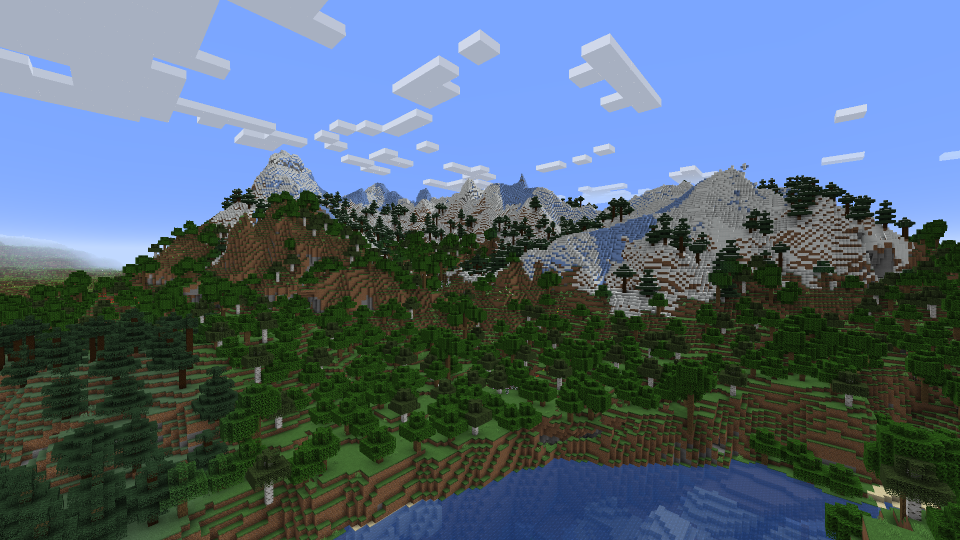
\includegraphics[width=0.8\textwidth]{figuras/minecraft_world.png}
	}{
		\Fonte{Disponível em: \url{https://minecraft.wiki/w/World\_generation}. Acesso em: 23 jan. 2026.}
	}
\end{figure}

\subsection{Vantagens e Desafios da \texorpdfstring{\gls{PCG}}{PCG}}
\label{subsec:vantagens_desafios_pcg}

A adoção da \gls{PCG} no desenvolvimento de jogos traz consigo um conjunto de
vantagens significativas, mas também impõe desafios consideráveis que precisam
ser gerenciados pelos desenvolvedores. Entre as principais vantagens, figura a
capacidade de oferecer alta rejogabilidade \cite{lazaridis2024creating}. A
\gls{PCG} permite a criação de mundos vastos e variados que seriam inviáveis de
serem construídos manualmente, como observado em \textit{No Man's Sky}. Outro
benefício importante é a eficiência de armazenamento, já que o conteúdo é gerado
em tempo de execução ou durante o desenvolvimento a partir de algoritmos
compactos, em vez de armazenar grandes volumes de dados pré-fabricados.
Adicionalmente, a \gls{PCG} possui o potencial para adaptação dinâmica do
conteúdo às ações ou ao perfil do jogador, criando experiências mais
personalizadas.

Contudo, a \gls{PCG} não está isenta de desafios. O controle de qualidade do
conteúdo gerado pode ser complexo, pois é preciso garantir que os resultados
sejam consistentemente bons, esteticamente agradáveis e livres de artefatos
indesejados ou bugs \cite{lazaridis2024creating}. A garantia de jogabilidade,
incluindo a solvabilidade níveis ou quebra-cabeças e a "justiça"\ das situações
de jogo, é outra preocupação central; um nível gerado proceduralmente deve ser
sempre solucionável e oferecer um desafio adequado. A previsibilidade excessiva
pode minar a sensação de descoberta, enquanto a aleatoriedade descontrolada pode
gerar conteúdo incoerente ou frustrante.  Finalmente, um dos desafios mais
debatidos é a dificuldade em replicar o "toque humano", ou seja, criar conteúdo
com significado profundo, intenção autoral forte ou nuances emocionais complexas
que são frequentemente associadas ao design manual \cite{lazaridis2024creating}.

\subsection{Técnicas Comuns de \texorpdfstring{\gls{PCG}}{PCG}}
\label{subsec:tecnicas_pcg}

O campo da \gls{PCG} abrange uma diversidade de técnicas algorítmicas, cada uma
com suas particularidades e aplicabilidades. Para a geração de níveis, foco
deste trabalho, e também para narrativas simples, algumas abordagens se destacam
antes da introdução de \gls{LLM}s, que serão discutidos posteriormente. É
importante ressaltar que muitas dessas técnicas podem ser combinadas para
alcançar resultados mais complexos e controláveis.

Algoritmos baseados em ruído, como \textit{Perlin Noise} \cite{perlin1985image}
e \textit{Simplex Noise} \cite{Perlin2001Noise}, são frequentemente utilizados
para gerar terrenos, texturas, mapas de altura e outras distribuições espaciais
que requerem uma aparência orgânica e natural. Esses algoritmos produzem padrões
pseudoaleatórios que podem ser parametrizados para controlar características
como frequência e amplitude, resultando em formações geográficas verossímeis ou
distribuições de recursos. Um exemplo prático disso pode ser observado na
Figura~\ref{fig:minecraft_biomes}, que ilustra as funções de densidade (com
\textit{3D noise}) utilizadas na geração de biomas e altura de terreno no jogo
\textit{Minecraft}.

\begin{figure}[!ht]
	\centering
	\Caption{\label{fig:minecraft_biomes} Exemplo de funções de densidade que
		utilizam ruído 3D para geração de biomas e altura de terreno no
		\textit{Minecraft}}
	\UFCfig{}{
		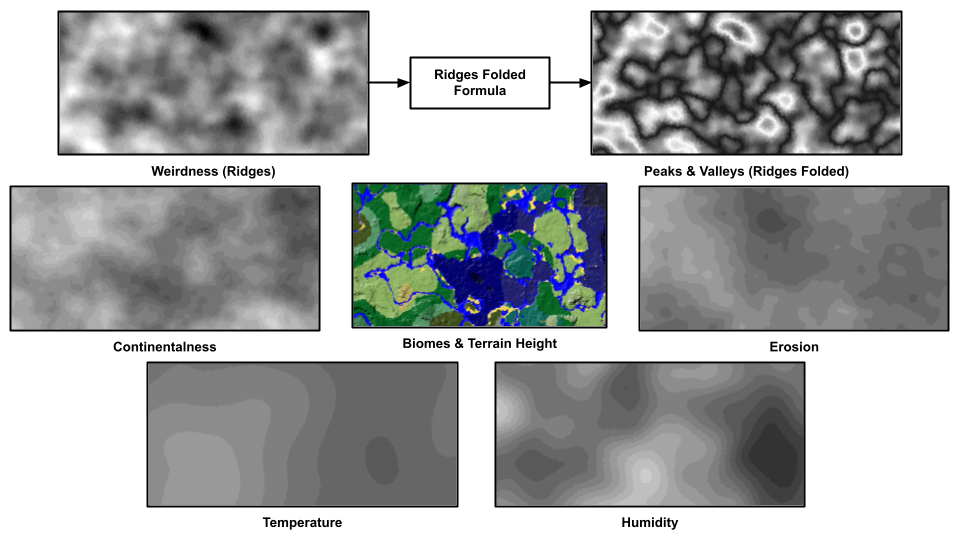
\includegraphics[width=0.8\textwidth]{figuras/minecraft_density_functions.png}
	}{
		\Fonte{Disponível em: \url{https://minecraft.wiki/w/World\_generation}. Acesso em: 23 jan. 2026.}
	}
\end{figure}

Gramáticas formais, incluindo \textit{L-Systems}
\cite{lindenmayer1968mathematical}, \textit{Shape Grammars}
\cite{stiny1971shape} e \textit{Graph Grammars} \cite{ehrig1973graph}, oferecem
um meio poderoso para definir regras de construção que podem gerar estruturas
complexas e recursivas. L-Systems são notáveis para modelar o crescimento de
plantas e fractais. Shape Grammars operam sobre formas geométricas, permitindo a
criação de estilos arquitetônicos ou layouts. Graph Grammars, particularmente
relevantes para a geração de níveis em jogos do tipo \textit{roguelike},
manipulam grafos para definir a estrutura e conectividade de salas, corredores e
áreas em um mapa, como pode ser observado na Figura~\ref{fig:mapa_grafo}.

\begin{figure}[!ht]
	\centering
	\Caption{\label{fig:mapa_grafo} Exemplo de mapa gerado utilizando gramáticas
		de grafos}
	\UFCfig{}{
		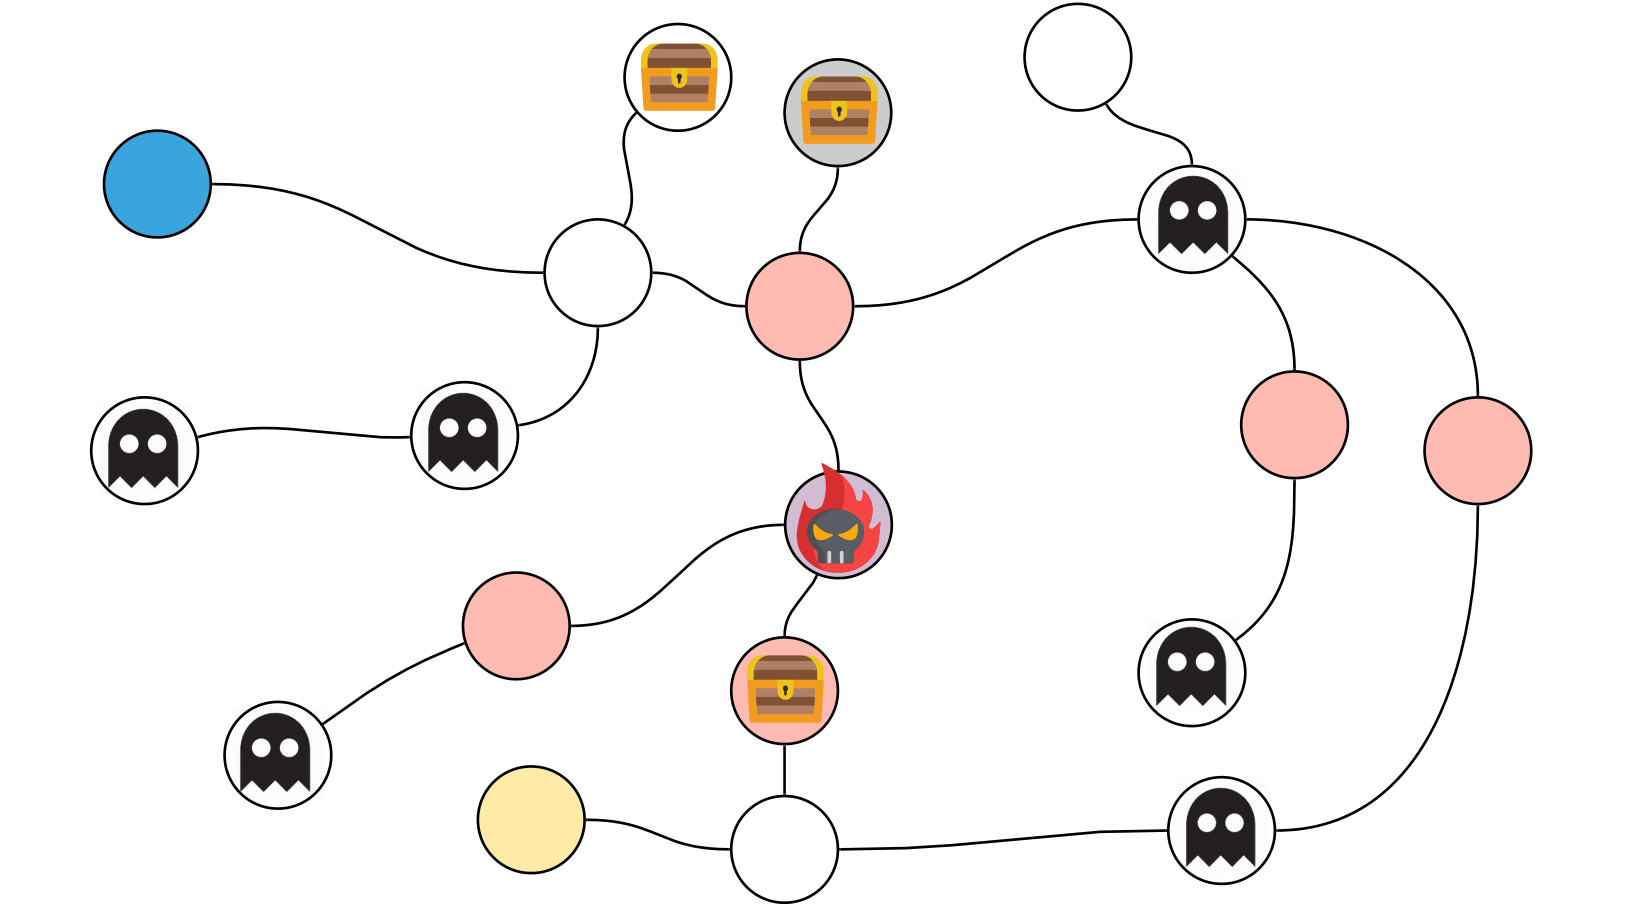
\includegraphics[width=0.8\textwidth]{figuras/mapa_gramatica_grafos.png}
	}{
		\Fonte{\cite{souza2019geraccao}}
	}
\end{figure}

Técnicas baseadas em agentes e simulação permitem que entidades autônomas
"esculpam"\ o ambiente ou distribuam elementos a partir de suas interações,
criando padrões complexos. Um exemplo clássico é o algoritmo \textit{Random
	Walk} \cite{pearson1905problem}, no qual um agente se move aleatoriamente por uma
grade, "cavando"\ túneis ou caminhos, frequentemente usado na geração de
cavernas ou masmorras simples \cite{koesnaedi2022implementation}. Simulações
mais complexas podem envolver múltiplos agentes com comportamentos distintos
para criar ecossistemas ou padrões urbanos.

A \gls{PCG} \textit{Search-Based} \cite{togelius2011search} utiliza algoritmos
de otimização, como algoritmos genéticos, evolução diferencial ou
\textit{simulated annealing}, para explorar o vasto espaço de possíveis
conteúdos e encontrar aqueles que melhor satisfazem um conjunto de critérios de
qualidade ou restrições de design, definidos por uma função de avaliação. Esta
abordagem é útil quando o designer tem objetivos claros sobre as propriedades
desejadas do conteúdo, mas a geração direta é complexa.

Finalmente, abordagens baseadas em Aprendizado de Máquina, anteriores à
proeminência dos \gls{LLM}s, já exploravam a capacidade de aprender padrões a
partir de dados de exemplo para gerar novo conteúdo. Isso inclui técnicas como
\gls{ANN} \cite{mcculloch1943logical}, Árvores de Decisão
\cite{loh2011classification}, ou Cadeias de Markov \cite{levin2017markov} para
gerar sequências, como layouts de níveis, trechos de música ou comportamento de
inimigos. A ascensão dos \gls{LLM}s pode ser vista como uma evolução natural e
mais poderosa desta vertente, especialmente para conteúdo com estrutura
sequencial ou semântica complexa, como narrativas.

\section{\texorpdfstring{\gls{LLM}s}{LLMs}}
\label{sec:llms}

Os \gls{LLM}s representam uma classe de modelos de inteligência artificial que
demonstraram capacidades notáveis no processamento e geração de linguagem
natural. Sua ascensão tem sido impulsionada por avanços em arquiteturas de redes
neurais, disponibilidade de grandes volumes de dados textuais e poder
computacional crescente.

\subsection{Definição e Evolução Histórica dos \texorpdfstring{\gls{LLM}s}{LLMs}}
\label{subsec:definicao_evolucao_llms}

Os \gls{LLM}s são modelos de inteligência artificial treinados em vastas
quantidades de dados textuais, o que lhes confere a capacidade de entender,
gerar e manipular a linguagem humana de forma coerente e contextualmente
relevante \cite{hadi2023survey}. Eles são projetados para prever a próxima
palavra ou caractere em uma dada sequência de texto, uma tarefa fundamental no
\gls{NLP}.

A evolução dos \gls{LLM}s pode ser observada desde os primeiros modelos de linguagem
estatísticos, como \textit{n-grams} \cite{brown1992class}, que se baseavam em contagens
de frequência de sequências de palavras. Posteriormente, as \gls{RNN} e suas
variantes, como \gls{LSTM} \cite{hochreiter1997long}, trouxeram melhorias ao
capturar dependências de longo alcance no texto, embora ainda enfrentassem
desafios com sequências muito longas e paralelização do treinamento
\cite{hadi2023survey}.

Um marco fundamental nessa evolução foi a introdução da arquitetura Transformer
no artigo \textit{"Attention is All You Need"}\ por \citeonline{vaswani2017attention}.
Essa arquitetura, baseada unicamente em mecanismos de atenção, dispensou a
recorrência e permitiu um treinamento mais eficiente e paralelizável em grandes
volumes de dados. A partir dos Transformers, surgiram modelos influentes como
\gls{BERT} \cite{devlin2019bert} e a série \gls{GPT}
\cite{radford2018improving}, que estabeleceram novos paradigmas no \gls{NLP} e
impulsionaram o desenvolvimento dos \gls{LLM}s modernos \cite{hadi2023survey}.

\subsection{Transformers e Mecanismo de Atenção}
\label{subsec:arquitetura_transformers_atencao}

A arquitetura \textit{Transformer}, conforme introduzida por
\citeonline{vaswani2017attention}, é a base da maioria dos \gls{LLM}s
contemporâneos.  Diferentemente das arquiteturas baseadas em \gls{RNN} ou
\gls{CNN} \cite{lecun1998gradient}, os Transformers processam todos os
\textit{tokens}\footnote{Um \textit{token} pode ser uma palavra, uma subpalavra (um subconjunto de
	uma palavra) ou até mesmo um único caractere.  Fonte (Acesso em: 23 jan. 2026):
	\url{https://developers.google.com/machine-learning/crash-course/llm/transformers}} de
uma sequência de entrada simultaneamente, o que facilita a paralelização e o
treinamento em hardware especializado como \gls{GPU} e \gls{TPU}
\cite{lin2022survey}.

Um dos seus componentes mais revolucionários é o mecanismo de
\textit{self-attention}. Este mecanismo permite que o modelo, ao processar uma
\textit{token} em uma sequência, pondere a importância de todos os outros
\textit{tokens} na mesma sequência. Essencialmente, ele calcula "scores de
atenção"\ que determinam o quanto cada palavra deve contribuir para a
representação da palavra atual. Isso possibilita que o modelo capture
dependências de longo alcance e entenda o contexto de forma mais eficaz, mesmo
em sequências de texto extensas \cite{vaswani2017attention,
	naveed2023comprehensive}. A capacidade de processar sequências em paralelo,
combinada com o poder do mecanismo de auto-atenção para modelar relações
contextuais complexas, tornou os \textit{Transformers} particularmente adequados para o
treinamento em grandes volumes de dados textuais, resultando nas capacidades
impressionantes dos \gls{LLM}s atuais \cite{lin2022survey}.

\subsection{Treinamento e Capacidades dos \texorpdfstring{\gls{LLM}s}{LLMs}}
\label{subsec:treinamento_capacidades_llms}

O treinamento de \gls{LLM}s geralmente envolve duas fases principais. A primeira
é o pré-treinamento, no qual o modelo é exposto a enormes quantidades de dados
textuais não rotulados (tais como, livros, artigos, websites). Durante essa fase, o
modelo aprende a prever palavras mascaradas em uma sentença (como no \gls{BERT})
ou a próxima palavra em uma sequência (como no \gls{GPT}), o que o força a
aprender padrões linguísticos, conhecimento de mundo e relações semânticas
complexas \cite{liu2024understanding, naveed2023comprehensive}.

Após o pré-treinamento, os modelos podem passar por um processo de ajuste
\textit{fine-tuning} para tarefas específicas. Nesta etapa, o modelo
pré-treinado é treinado adicionalmente em um dataset menor e específico da
tarefa (por exemplo, tradução, sumarização, resposta a perguntas), com dados
rotulados.  Isso adapta o conhecimento geral adquirido durante o pré-treinamento
para a tarefa desejada \cite{liu2024understanding}.

Como resultado, os \gls{LLM}s exibem uma vasta gama de capacidades, incluindo a
geração de texto coerente e criativo, tradução entre idiomas, sumarização de
documentos longos, resposta a perguntas de forma informativa, e até mesmo a
escrita de código \cite{hadi2023survey}. Uma característica notável é a
emergência de capacidades complexas, como o raciocínio em múltiplos passos e o
aprendizado em poucos exemplos (\textit{few-shot learning}) ou mesmo sem
exemplos prévios (\textit{zero-shot learning}), no qual o modelo pode realizar
tarefas para as quais não foi explicitamente treinado, apenas com base em uma
descrição da tarefa e, opcionalmente, alguns exemplos fornecidos no prompt
\cite{vaswani2017attention, naveed2023comprehensive}.

\subsection{\texorpdfstring{\gls{LLM}s}{LLMs} Aplicados à \texorpdfstring{\gls{PCG}}{PCG}}
\label{subsec:llms_pcg}

As capacidades dos \gls{LLM}s, especialmente sua proficiência na compreensão e
geração de linguagem natural, alinham-se de forma promissora com as necessidades
da \gls{PCG} em jogos \cite{maleki2024procedural}. A \gls{PCG} visa criar
conteúdo de jogo (níveis, narrativas, itens, etc.) algoritmicamente, e os
\gls{LLM}s oferecem novas possibilidades para enriquecer e personalizar esse
processo.

Um dos potenciais mais diretos dos \gls{LLM}s na \gls{PCG} é a geração de
elementos textuais. Isso inclui a criação de narrativas dinâmicas que se adaptam
às ações do jogador, diálogos interativos e realistas para \gls{NPC}s, descrições
ricas e detalhadas de itens, locais e personagens, e histórias de fundo para o
mundo do jogo \cite{rolim2023llms}. A capacidade dos \gls{LLM}s
de manter a coerência e o contexto ao longo de textos extensos é particularmente
valiosa para esses fins.

\begin{figure}[!ht]
	\centering
	\Caption{\label{fig:mariogpt_arch} Arquitetura do sistema \textit{MarioGPT}. Um
		prompt textual é processado por um encoder de texto, cujas saídas são usadas
		em um mecanismo de atenção cruzada com as camadas \gls{GPT}. As camadas
		\gls{GPT} também recebem um nível "tokenizado"\ inicial. O sistema então prediz
		a continuação do nível "tokenizado", que é convertido para um nível de jogo
		visual.}
	\UFCfig{}{
		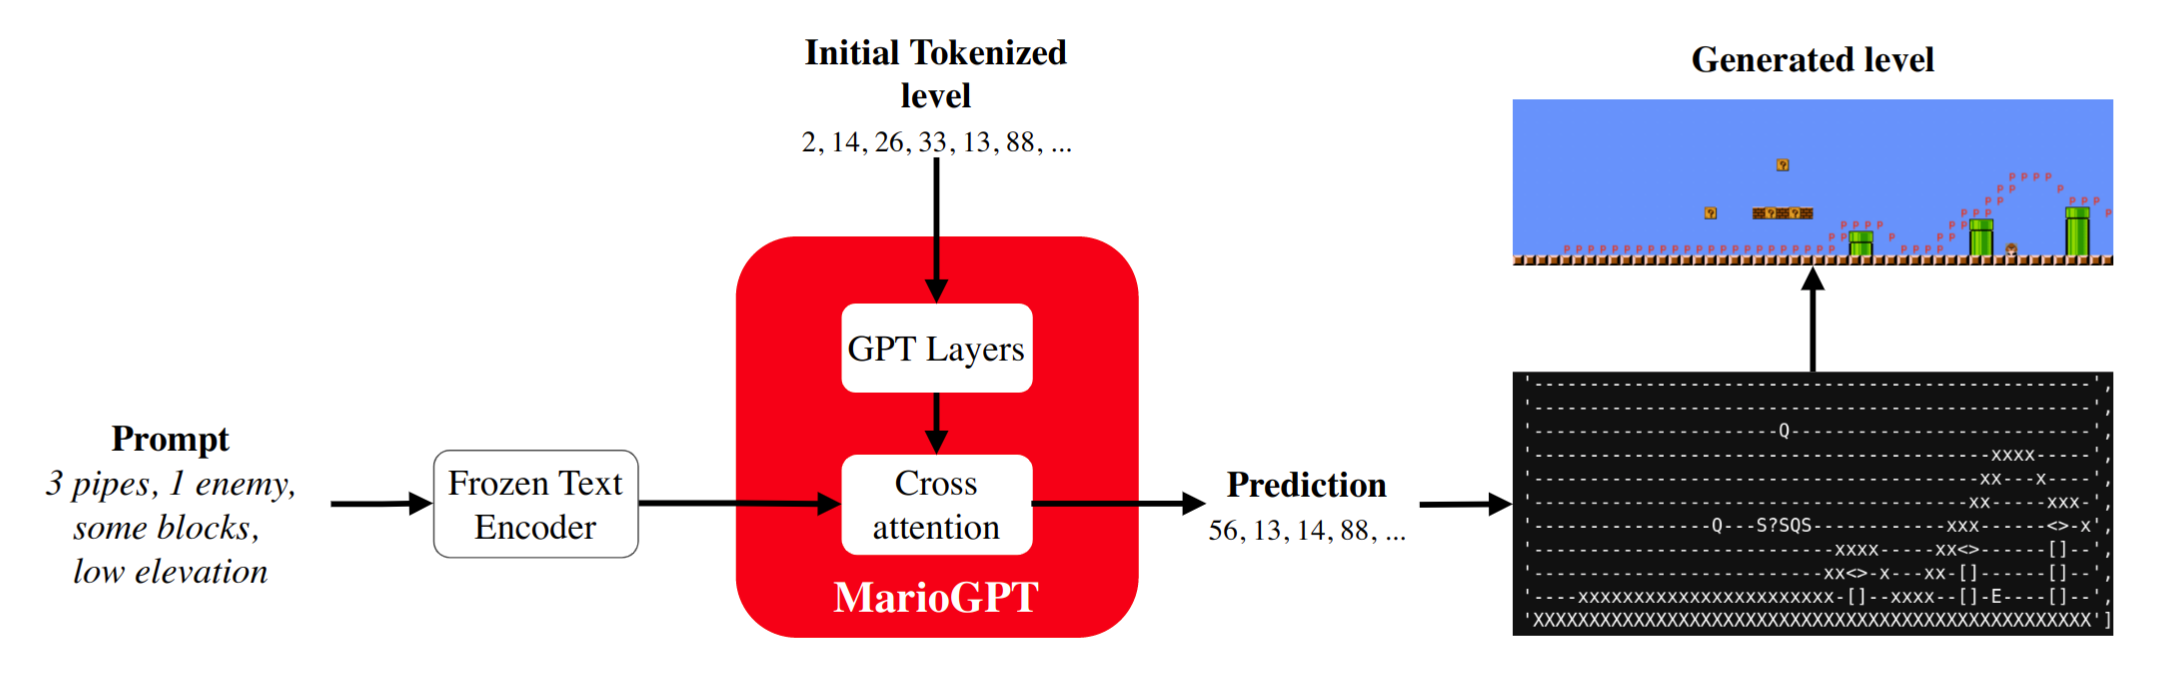
\includegraphics[width=0.8\textwidth]{figuras/mario_gpt.png}
	}{
		\Fonte{\cite{sudhakaran2023mariogpt}}
	}
\end{figure}

Além de elementos puramente textuais, os \gls{LLM}s também têm potencial para
influenciar a geração de elementos estruturais, ainda que indiretamente. Por
exemplo, um \gls{LLM} pode gerar descrições textuais detalhadas de
\textit{layouts} de níveis, sequências de eventos de uma missão, ou regras de um
sistema de jogo. Essas descrições podem então ser interpretadas por outros
sistemas ou algoritmos de \gls{PCG} para traduzi-las em conteúdo de jogo
concreto \cite{maleki2024procedural}.  Pesquisas recentes, como o projeto
\textit{MarioGPT} (cuja arquitetura é ilustrada na Figura~\ref{fig:mariogpt_arch}),
exploraram o uso de \gls{LLM}s para gerar níveis de jogos 2D a partir de
\textit{prompts} textuais, indicando um caminho para a personalização de
conteúdo de jogo com base nas preferências do usuário expressas em linguagem
natural.
